\documentclass{beamer}
\usepackage{listings}

\title{Scalable N-Body Event Prediction}
\author
{Steven Braeger \and Nick Arnold}
\institute
{
  \inst{1}%
  University of Central Florida
}
\date
{\today}

\begin{document}

\frame{\titlepage}

\begin{frame}
	\frametitle{Discrete Event Simulation}
	\begin{itemize}
		\item Video games and real time simulation
		\begin{itemize}
			\item Large scale parallel clusters
			\item Massively parallel GPU architectures
		\end{itemize}
		\item Evolution of systems of dynamic and static objects
		\begin{itemize}
			\item Dynamic objects physically collide with other objects
			\item Model and react to collisions
		\end{itemize}
		\item Simple demo
	\end{itemize}
\end{frame}

\begin{frame}[fragile]
	\frametitle{Naive Implementation}
	\begin{itemize}
		\item Embarrasingly parallel implementation
		\begin{itemize}
			\item Busy-wait loop
			\item Objects are continually polled, waiting for collisions
		\end{itemize}
		\item
	\begin{lstlisting}[language=C,basicstyle=\footnotesize,frame=single,tabsize=4,title=Naive\_Algorithm]
for each timestep ti do
    for each dynamic object do do
        update(do, dt) {dt is the constant timestep difference}
        for each object o do
            if check(do, o) then
                collide(do, o, dt)
            end if
        end for
    end for
end for
	\end{lstlisting}
		\item Allows thread per object or pair
		\item Wasteful, runs in $O(n ^ 2)$ time 
		\item In sufficiently large scenes, collisions are rare
		\begin{itemize}
			\item Vast majority of checks will fail
			\item How can we avoid making unneccessary checks?
		\end{itemize}
	\end{itemize}

\end{frame}

\begin{frame}[fragile]
	\frametitle{Our Proposed Predictive Algorithm}
	\begin{itemize}
		\item Instead of checking all possible object pairs for collisions, compute when pairs are likely to collide
		\begin{itemize}
			\item Based on physical computation using position, velocity, and acceleration
		\end{itemize}
		\item Store each pair's potential collision times into event queue
		\item
	\begin{lstlisting}[language=C,basicstyle=\footnotesize,frame=single,tabsize=4,title=Predictive\_Algorithm]
{initialize events from initial states}
for each timestep ti do
  for each dynamic object do do
    update(do, dt) {dt is the constant timestep difference}
  end for
  {for each event that occurs in this timestep}
  for each e in events.find(ti) do
    for each object o do
      if check(e.o, o) then
        collide(e.o, o, dt) {predict next collision event into queue}
      end if
    end for
    events.remove(e)
  end for
end for
return events

	\end{lstlisting}
	\item In worst case, also runs $O(n ^ 2)$ (initial population of event queue)
	\item Timesteps now see $O(n)$ search of event queue
	\item If collision, only recompute $2n$ future collisions
	\item Average case $O(n)$ behavior.
	\end{itemize}

\end{frame}

\begin{frame}
  \frametitle{Whiteboard Demonstration}
\end{frame}


\begin{frame}
	\frametitle{Potential Algorithm Issues}
	\begin{itemize}
		\item Predictive algorithm is not currently parallelizable
		\begin{itemize}
			\item Relies on independent accesses to global future event queue (shared state)
			\item Can we divide threads to ensure no collisions?
			\item Can we guarantee threads will all act on one timestep at a time?
		\end{itemize}
	\end{itemize}
\end{frame}

\begin{frame}
	\frametitle{Scalable Lock-Free Implementation}
	\begin{itemize}
		\item Reimplement algorithm using barriers and hardware atomic compare-and-swap primitives
		\begin{itemize}
			\item Guarantee thread safety
			\item Synchronizes threads utilizing the event queue
			\item Use array with thread-safe indexing scheme
			\item Uses subphase barriers to 
		\end{itemize}
	\end{itemize}
\end{frame}

\begin{frame}[fragile]
	\frametitle{Barriers}
	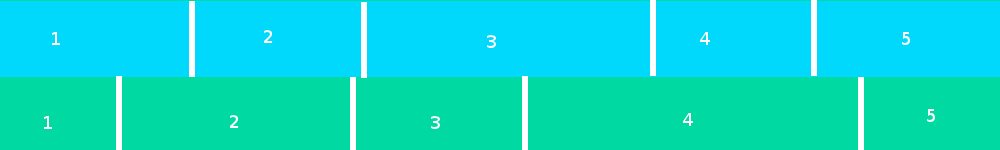
\includegraphics[width=.9\textwidth]{unsync.png}
	\begin{itemize}
		\item Barriers make threads wait until all threads have reached the barrier
		\item Then all threads are released to continue
		\item Allows us to partition simulation into frames.
		\item One timestep at a time.
		\item Argument: Barriers obey lock-free property
	\end{itemize}
	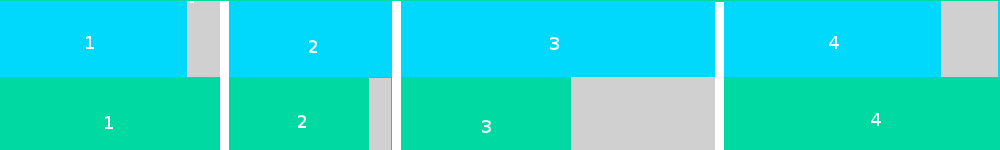
\includegraphics[width=.9\textwidth]{sync.png}
\end{frame}

\begin{frame}
	\frametitle{Future Event Queue}
	\begin{itemize}
	\item \emph{insert(event)} inserts an event into the queue, possibly superceding any events that happen later
	\item \emph{remove(event)} removes an event from the queue	
	\item \emph{find(time)} returns an iterator that iterates over all predicted events that occur after time $t$.
	\item \emph{find\_invalud()} Returns all objects for which nothing is known about their behavior
	\end{itemize}
\end{frame}

\begin{frame}
      \frametitle{Future Event Queue Implementation}
      \begin{itemize}
      \item Could use priority queue, but thread-safety problems.
       \item ObjectID indexed array.  One ``pending event'' per object
        \item Operations only operate on assigned object hashes
	\item insert(e) overwrites pending\[e.o1.id\] $O(1)$
	\item remove(e) invalidates pending\[e.o1.id\] $O(1)$
	\item find\_invalid() is a linear search through array $O(n)$
	\item find(t) is linear search $O(n)$
      \end{itemize}
\end{frame}


\begin{frame}
	\frametitle{Scalable Timestep Subphases}
	\begin{itemize}
		\item Our implementation can be divided into subphases
		\begin{itemize}
			\item check\_react\_collisions()
			\item repredict()
			\item update\_simulation()
			\item timestep\_sync\_barrier.wait()
		\end{itemize}
		\item Important to not allow different threads in different subphases at the same time
		\item Implement subphase barriers as well...3*3 cases of overlap behavior->3 cases
	\end{itemize}
\end{frame}

\begin{frame}[fragile]
	\frametitle{Updating Objects}
	\begin{itemize}
		\item Updating each object's position requires no information for any other objects
		\item Physical motion calculation
		\item Can be done in parallel without worry of collision
		\item Reads/Writes only thread owned object
	\begin{lstlisting}[language=C,basicstyle=\footnotesize,frame=single,tabsize=4,title=Update]
for every object o assigned to current thread do
  update(o)
end for
	\end{lstlisting}
	\end{itemize}
\end{frame}
\begin{frame}[fragile]
	\frametitle{Check React Collisions (cont.)}
	\begin{lstlisting}[language=C,basicstyle=\footnotesize,frame=single,tabsize=4,title=Check\_React\_Collisions]
{search event queue for events that are occuring now}
for e in events.find(current time) do
  {if object reacted yet is false,set reacted to true and do the event}
  if !compare and exchange(reacted yet[e.o1],false,true)
  then
    {if the event hasn’t been happens and this thread is assigned to it}
    if e.o1 is in current thread and check(e.o1, e.o2) then
      {modify both objects}
      collide(e.o1, e.o2)
    end if
    {the event is passed, so remove it.}
    events.remove(e)
  end if
end for
	\end{lstlisting}
\end{frame}
\begin{frame}
	\frametitle{Check React Collisions}
	\begin{itemize}
		\item Potential synchronization issues
		\begin{itemize}
			\item Collide() method reads and writes TWO objects, which could be assigned to other threads non-deterministically
			\item Two events in the event queue could be describing the same collision from different perspectives
			\item Multiple threads could check an object while another thread is writing to it
		\end{itemize}
		\item Solved by adding a flag bit
		\item Flag determines whether object has been collided this timestep
	\end{itemize}
\end{frame}

\begin{frame}[fragile]
	\frametitle{Repredict Collisions}
	\begin{itemize}
		\item Recalculate future collisions for invalidated pairs
		\begin{itemize}
			\item Collisions that just occurred
			\item Collisions that were checked, but did not occur
		\end{itemize}
		\item This step may read objects belonging to other threads, but won't modify them
		\item
	\begin{lstlisting}[language=C,basicstyle=\footnotesize,frame=single,tabsize=4,title=Repredict]
{search event queue for objects that the queue is unaware of}
for oinvalid in events.find invalid(current time) do
  {if invalid object is assigned to this thread}
  if oinvalid in current thread then
    for all dynamic objects do do
      events.insert(predict(oinvalid, do))
    end for
  end if
end for
	\end{lstlisting}
	\end{itemize}
\end{frame}

\begin{frame}
	\frametitle{Results}
	\begin{center}
		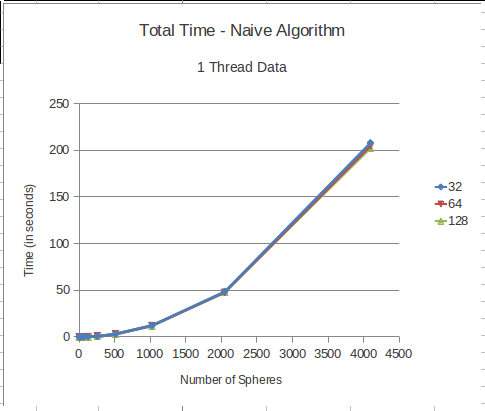
\includegraphics[width=.75\textwidth]{runtime_naive_1thread.png}
	\end{center}
\end{frame}

\begin{frame}
	\frametitle{Results (cont.)}
	\begin{center}
		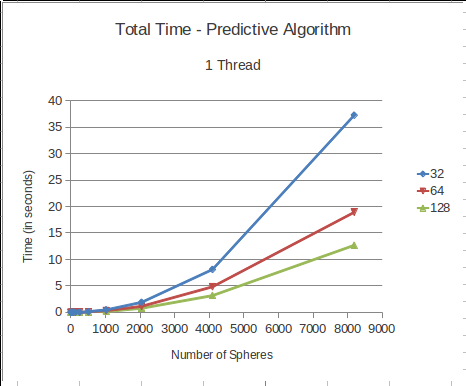
\includegraphics[width=.75\textwidth]{runtime_predictive_1thread.png}
	\end{center}
\end{frame}

\begin{frame}
	\frametitle{Results (cont.)}
	\begin{center}
		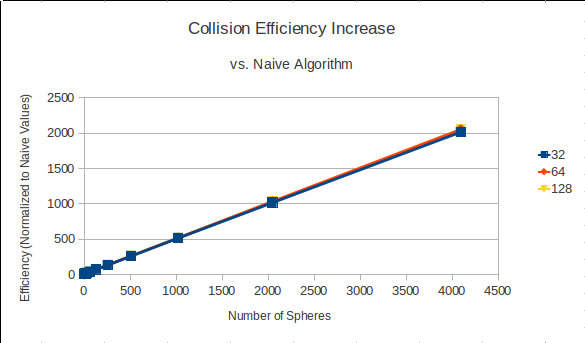
\includegraphics[width=.75\textwidth]{collision_efficiency.png}
	\end{center}
\end{frame}

\begin{frame}
	\frametitle{Results (cont.)}
	\begin{center}
		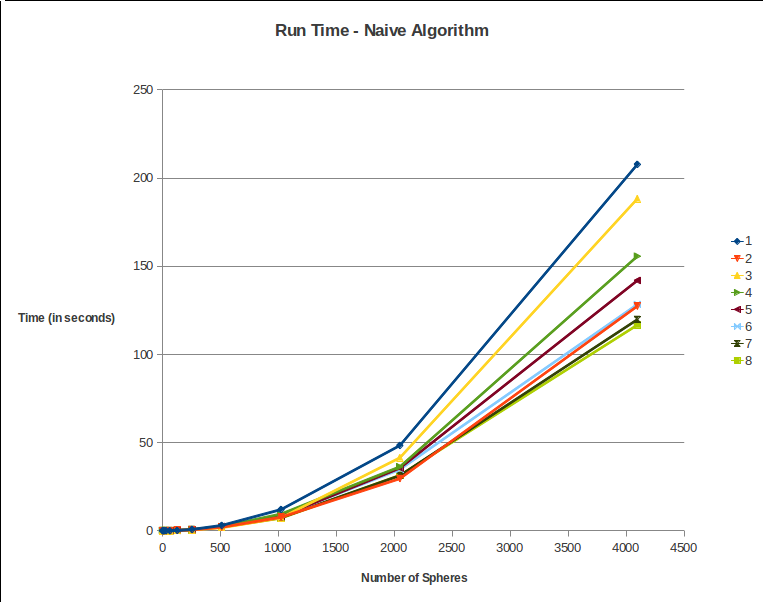
\includegraphics[width=.75\textwidth]{runtime_naive_allthreads.png}
	\end{center}
\end{frame}

\begin{frame}
	\frametitle{Results (cont.)}
	\begin{center}
		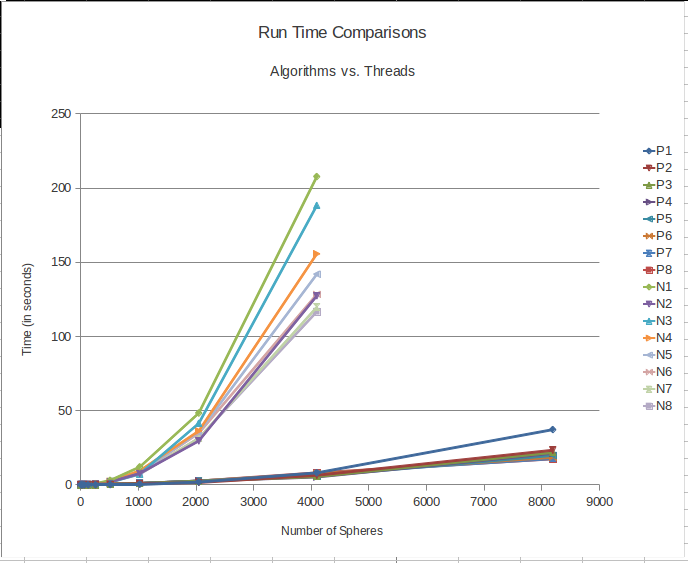
\includegraphics[width=.75\textwidth]{runtime_comparison.png}
	\end{center}
\end{frame}

\begin{frame}
	\frametitle{Results (cont.)}
	\begin{center}
		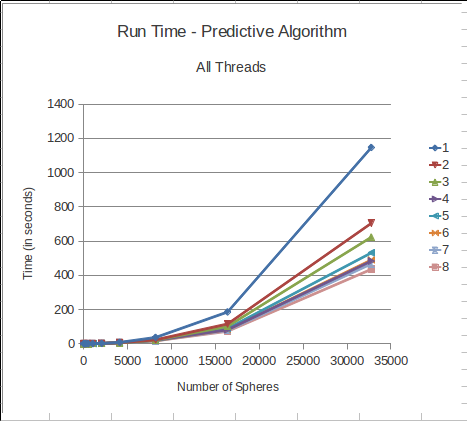
\includegraphics[width=.75\textwidth]{runtime_predictive_allthreads.png}
	\end{center}
\end{frame}

\begin{frame}
	\frametitle{Results (cont.)}
	\begin{center}
		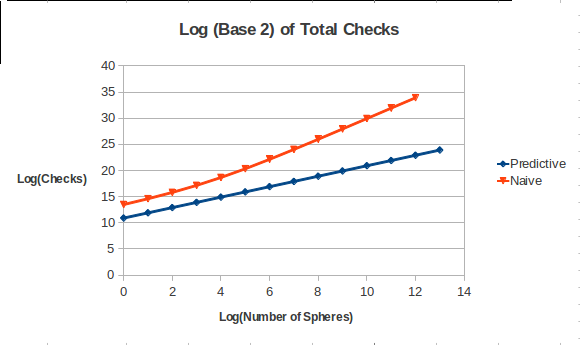
\includegraphics[width=.75\textwidth]{log_total_checks_comparison.png}
	\end{center}
\end{frame}

\begin{frame}
	\frametitle{Results (cont.)}
	\begin{center}
		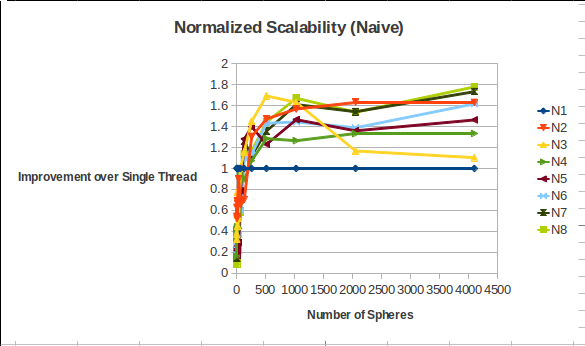
\includegraphics[width=.75\textwidth]{normalized_scalability_naive.png}
	\end{center}
\end{frame}

\begin{frame}
	\frametitle{Results (cont.)}
	\begin{center}
		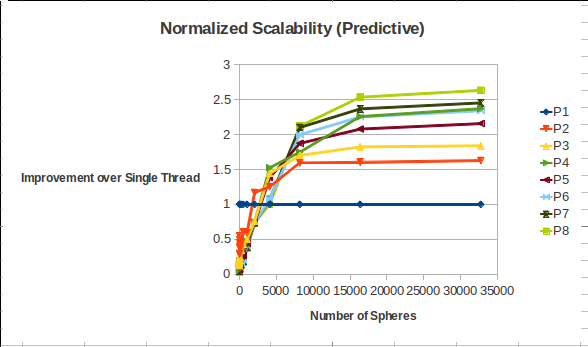
\includegraphics[width=.75\textwidth]{normalized_scalability_predictive.png}
	\end{center}
\end{frame}m


\begin{frame}
  \frametitle{Questions?}
\end{frame}



	
\end{document}
